%%%
%% This is file `sample-sigplan.tex',
%% generated with the docstrip utility.
%%
%% The original source files were:
%%
%% samples.dtx  (with options: `sigplan')
%%
%% IMPORTANT NOTICE:
%%
%% For the copyright see the source file.
%%
%% Any modified versions of this file must be renamed
%% with new filenames distinct from sample-sigplan.tex.
%%
%% For distribution of the original source see the terms
%% for copying and modification in the file samples.dtx.
%%
%% This generated file may be distributed as long as the
%% original source files, as listed above, are part of the
%% same distribution. (The sources need not necessarily be
%% in the same archive or directory.)
%%
%%
%% Commands for TeXCount
%TC:macro \cite [option:text,text]
%TC:macro \citep [option:text,text]
%TC:macro \citet [option:text,text]
%TC:envir table 0 1
%TC:envir table* 0 1
%TC:envir tabular [ignore] word
%TC:envir displaymath 0 word
%TC:envir math 0 word
%TC:envir comment 0 0
%%
%%
%% The first command in your LaTeX source must be the \documentclass command.
%%\documentclass[sigplan,nonacm]{acmart}
%%\documentclass[sigplan, nonacm]{acmart}\settopmatter{printfolios=true,printccs=false,printacmref=false}
\documentclass[acmsmall,nonacm]{acmart}\settopmatter{printfolios=true,printccs=false,printacmref=false}

\graphicspath{{pictures/}}
%%
%% \BibTeX command to typeset BibTeX logo in the docs
\AtBeginDocument{%
	\providecommand\BibTeX{{%
			\normalfont B\kern-0.5em{\scshape i\kern-0.25em b}\kern-0.8em\TeX}}}

%% Rights management information.  This information is sent to you
%% when you complete the rights form.  These commands have SAMPLE
%% values in them; it is your responsibility as an author to replace
%% the commands and values with those provided to you when you
%% complete the rights form.
%%\setcopyright{acmcopyright}
\setcopyright{none}
%%\acmJournal{PACMPL}
%%\acmVolume{1}
%%\acmNumber{CONF} % CONF = POPL or ICFP or OOPSLA
%%\acmArticle{1}
%%\acmYear{2021}
%%\acmMonth{9}
%%\acmDOI{}
%%\copyrightyear{2018}
%%\acmYear{2018}
%%\acmDOI{10.1145/1122445.1122456}

%% These commands are for a PROCEEDINGS abstract or paper.
%%\acmConference[Woodstock '18]{Woodstock '18: ACM Symposium%% on Neural
%%  Gaze Detection}{June 03--05, 2018}{Woodstock, NY}
%%\acmBooktitle{Woodstock '18: ACM Symposium on Neural Gaze Detection,
%%  June 03--05, 2018, Woodstock, NY}
%%\acmPrice{15.00}
%%\acmISBN{978-1-4503-XXXX-X/18/06}


%%
%% Submission ID.
%% Use this when submitting an article to a sponsored event. You'll
%% receive a unique submission ID from the organizers
%% of the event, and this ID should be used as the parameter to this command.
%%\acmSubmissionID{123-A56-BU3}

%%
%% The majority of ACM publications use numbered citations and
%% references.  The command \citestyle{authoryear} switches to the
%% "author year" style.
%%
%% If you are preparing content for an event
%% sponsored by ACM SIGGRAPH, you must use the "author year" style of
%% citations and references.
%% Uncommenting
%% the next command will enable that style.
%%\citestyle{acmauthoryear}
\usepackage{xspace}
\usepackage{booktabs}   %% For formal tables:
                        %% http://ctan.org/pkg/booktabs
\usepackage{subcaption} %% For complex figures with subfigures/subcaptions
                        %% http://ctan.org/pkg/subcaption

\usepackage[utf8]{inputenc}
\usepackage[T1]{fontenc}
\usepackage[scaled=0.78]{beramono}
\usepackage{amsmath}
\usepackage{mathtools}
\usepackage{stmaryrd}
%\usepackage{unicode-math}
%\usepackage{MnSymbol}
\usepackage{wasysym}
\usepackage{color}
\usepackage{xcolor,colortbl}
\usepackage{url}
\usepackage{listings}
\usepackage{paralist}
%\usepackage[compact]{titlesec}
\usepackage[font={small}]{caption}
\usepackage{wrapfig}
\usepackage{enumitem}
\usepackage{multicol}
\usepackage{multirow}
\usepackage{makecell}
\usepackage{flushend}
\usepackage{bcprules}
\usepackage{textcomp}
\usepackage{tikz}
\usetikzlibrary{positioning,fit,calc,arrows.meta,arrows,decorations}
\usepackage{pdfpages}
\usepackage{cleveref}
\usetikzlibrary{matrix}
\usepackage{xspace}
\definecolor{light-gray}{gray}{0.85}
\usepackage{stackengine}
\usepackage{mathpartir}
\usepackage{float}
\usepackage{bcprules}
\usepackage{semantic, stmaryrd}
% ----- listings

%\definecolor{ckeyword}{HTML}{7F0055}
\definecolor{ckeyword}{HTML}{000000}
\definecolor{ccomment}{HTML}{3F7F5F}
\definecolor{cstring}{HTML}{2A0099}

\lstdefinelanguage{Scala}%
{morekeywords={
  abstract, sealed, lazy,
  case,catch,char,class,%
  def,do,else,extends,final,finally,for,%
  if,import,implicit,%
  match,module,%
  new,null,undefined,%
  %fun,
  array,
  override,%
  package,private,protected,public,%
  for,public,return,super,%
  this,throw,trait,try,type,%
  val,var,%
  with,while,%
  object,
  let,skip,assert,then,fst,snd,idx,sum,prod,exists,forall,%
  yield,%
  % some scheme keywords
  define, null?, car, cdr
  },%
  sensitive,%
  moredelim=*[il][\bfseries]{\#\#\ },
  morecomment=[l]//,%
  morecomment=[s]{/*}{*/},%
  morestring=[b]",%
  %morestring=[b]',%
  showstringspaces=false%
}[keywords,comments,strings]%

\lstdefinelanguage{Effect}%
{morekeywords={
    effect, yield, return
  },%
  sensitive,%
  moredelim=*[il][\bfseries]{\#\#\ },
  morecomment=[l]//,%
  morecomment=[s]{/*}{*/},%
  morestring=[b]",%
  %morestring=[b]',%
  showstringspaces=false%
}[keywords,comments,strings]%

\lstdefinelanguage{LLVM}%
{morekeywords={
    define, i32, br, icmp, sub, call, mul, phi, ret, label
  },%
  sensitive,%
  moredelim=*[il][\bfseries]{\#\#\ },
  morecomment=[l];,%
  morecomment=[s]{/*}{*/},%
  morestring=[b]",%
  %morestring=[b]',%
  showstringspaces=false%
}[keywords,comments,strings]%

\lstdefinelanguage{CPP}%
{morekeywords={
    using, void, function, if, else, Cont, List
  },%
  sensitive,%
  moredelim=*[il][\bfseries]{\#\#\ },
  morecomment=[l]//,%
  morecomment=[s]{/*}{*/},%
  morestring=[b]",%
  %morestring=[b]',%
  showstringspaces=false%
}[keywords,comments,strings]%


\lstset{
  language=Scala,%
  mathescape=true,%
%  columns=[c]fixed,%
  aboveskip=2pt,%\smallskipamount,
  belowskip=1pt,%\negsmallskipamount,
  lineskip=-1pt,
  basewidth={0.6em, 0.5em},%
%  backgroundcolor=\color{listingbg},
  basicstyle=\ttfamily,
  keywordstyle=\keywordstyle,
  commentstyle=\commentstyle,
  stringstyle=\stringstyle,
%  xleftmargin=0.5cm
  literate={-->}{{$\to$}}2
           {->}{{$\mapsto$}}3
           {<-}{{$\leftarrow$}}2
           {=>}{{$\Rightarrow ~$}}2
           {|-}{{$\ts$}}2
           %{fun}{{$\lambda$}}1
           {idx}{{$\#$}}1
           {array(}{{$\langle.\rangle$(}}3
           {σ}{{$\sigma$}}1
           {ρ}{{$\rho$}}1
           {→}{{$\to$}}1
           {←}{{$\leftarrow$}}1
           {λ}{{$\lambda$}}1
           {α}{{$\alpha$}}1
           {⊔}{{$\sqcup$}}1
           {⊓}{{$\sqcap$}}1
           {⊑}{{$\sqsubseteq$}}1
           {⊤}{{$\top$}}1
           {⊥}{{$\bot$}}1
           {×}{{$\times$}}1
           {τ}{{$\tau$}}1
           {ψ}{{$\psi$}}1
           {Σ}{{$\Sigma$}}1
           {⟨}{{$\langle$}}1
           {⟩}{{$\rangle$}}1
           {π}{{$\pi$}}1
           {∪}{{$\cup$}}2
           %{[[}{{$[\![$}}1
           %{]]}{{$]\!]$}}1
           %{…}{{$\!...$}}1
}

\lstdefinestyle{small}{
  language=Scala,%
  mathescape=true,%
%  columns=[c]fixed,%
  aboveskip=2pt,%\smallskipamount,
  belowskip=1pt,%\negsmallskipamount,
  lineskip=-1pt,
  basewidth={0.6em, 0.45em},%
%  backgroundcolor=\color{listingbg},
  basicstyle=\fontsize{7}{9}\selectfont\ttfamily,
  keywordstyle=\keywordstyle,
  commentstyle=\commentstyle,
  stringstyle=\stringstyle,
%  xleftmargin=0.5cm
  literate={-->}{{$\to$}}3
           {->}{{$\mapsto$}}3
           {=>}{{$\Rightarrow ~$}}2
           {|-}{{$\ts$}}2
           %{fun}{{$\lambda$}}1
           {idx}{{$\#$}}1
           {sum}{{$\Sigma$}}1
           {array(}{{$\langle.\rangle$(}}3
           {σ}{{$\sigma$}}1
           {ρ}{{$\rho$}}1
           {→}{{$\to$}}1
           {λ}{{$\lambda$}}1
           {α}{{$\alpha$}}1
           {⊔}{{$\sqcup$}}1
           {⊓}{{$\sqcap$}}1
           {⊑}{{$\sqsubseteq$}}1
           {⊤}{{$\top$}}1
           {⊥}{{$\bot$}}1
           {×}{{$\times$}}1
           {τ}{{$\tau$}}1
           {ψ}{{$\psi$}}1
           %{[[}{{$[\![$}}1
           %{]]}{{$]\!]$}}1
           %{…}{{$\!...$}}1
}

\lstdefinestyle{extrasmall}{
  language=Scala,%
  mathescape=true,%
%  columns=[c]fixed,%
  aboveskip=2pt,%\smallskipamount,
  belowskip=1pt,%\negsmallskipamount,
  lineskip=-1pt,
  basewidth={0.6em, 0.45em},%
%  backgroundcolor=\color{listingbg},
  basicstyle=\fontsize{6}{8}\selectfont\ttfamily,
  keywordstyle=\keywordstyle,
  commentstyle=\commentstyle,
  stringstyle=\stringstyle,
%  xleftmargin=0.5cm
  literate={-->}{{$\to$}}3
           {->}{{$\mapsto$}}3
           {=>}{{$\Rightarrow ~$}}2
           {|-}{{$\ts$}}2
           %{fun}{{$\lambda$}}1
           {idx}{{$\#$}}1
           {sum}{{$\Sigma$}}1
           {array(}{{$\langle.\rangle$(}}3
           {σ}{{$\sigma$}}1
           {ρ}{{$\rho$}}1
           {→}{{$\to$}}1
           {λ}{{$\lambda$}}1
           {α}{{$\alpha$}}1
           {⊔}{{$\sqcup$}}1
           {⊓}{{$\sqcap$}}1
           {⊑}{{$\sqsubseteq$}}1
           {⊤}{{$\top$}}1
           {⊥}{{$\bot$}}1
           {×}{{$\times$}}1
           %{[[}{{$[\![$}}1
           %{]]}{{$]\!]$}}1
           %{…}{{$\!...$}}1
}

\lstdefinestyle{JavaScriptTiny}{
    style=JavaScript, % Inherit from the JavaScript style
    basicstyle=\ttfamily\tiny,
    numberstyle=\ttfamily\tiny, % Set the number style to \tiny
}

\lstdefinestyle{JavaScript}{
    language=java,
    basicstyle=\ttfamily\scriptsize,
    keywordstyle=\color{blue},
    commentstyle=\color{green!50!black},
    stringstyle=\color{black},
    showstringspaces=false,
    breaklines=true,
    breakatwhitespace=true,
    tabsize=1,
    numbersep=2pt,
    numberstyle=\ttfamily\tiny,
    % morekeywords={let, const, var, function, if, else, pipe, map, group, count, plus, minus,
    % while, for, return, typeof, switch, case, merge, get, sum, min, max, div, keyval, apply, times},
    morekeywords={let, const, var, function, if, else}
    escapeinside={(*@}{@*)}
}

\lstdefinestyle{JavaScriptInline}{
    language=java,
    basicstyle=\ttfamily\scriptsize,
    keywordstyle=\color{blue},
    commentstyle=\color{green!50!black},
    stringstyle=\color{black},
    showstringspaces=true,
    breaklines=true,
    breakatwhitespace=true,
    tabsize=1,
    numbersep=2pt,
    numberstyle=\ttfamily\tiny,
    morekeywords={},
    escapeinside={(*@}{@*)}
}

\lstset{style=JavaScript, upquote=true}

\lstdefinestyle{JSComment}{
    language=java,
    basicstyle=\color{green!50!black}\ttfamily\scriptsize,
    commentstyle=\color{green!50!black},
    showstringspaces=true,
    breaklines=true,
    breakatwhitespace=true,
    tabsize=1,
}

\definecolor{listingbg}{RGB}{240, 240, 240}

\newcommand{\commentstyle}[1]{\color{ccomment}\itshape{#1}}
\newcommand{\keywordstyle}[1]{\color{ckeyword}\bfseries{#1}}
%\newcommand{\keywordstyle}[1]{\color{ckeyword}{#1}}
%\newcommand{\stringstyle}[1]{\color{cstring}\bfseries{#1}}
\newcommand{\stringstyle}[1]{\color{cstring}\text{#1}}

\lstnewenvironment{listing}{\lstset{language=Scala}}{}
\lstnewenvironment{listingtiny}{\lstset{language=Scala,basicstyle=\scriptsize\ttfamily}}{}

\newcommand{\code}[1]{\lstinline[language=Scala,columns=fixed,basicstyle=\ttfamily]|#1|}

% ----- packed items, so we don't waste space
\newenvironment{sitemize}{
\begin{itemize}[leftmargin=2.5ex]
  \setlength{\itemsep}{1pt}
  \setlength{\parskip}{0pt}
  \setlength{\parsep}{0pt}
}{\end{itemize}}

\newenvironment{senumerate}{
\begin{enumerate}[leftmargin=2.5ex]
  \setlength{\itemsep}{1pt}
  \setlength{\parskip}{0pt}
  \setlength{\parsep}{0pt}
}{\end{enumerate}}

\newcommand{\mypar}[1]{{\bf #1.}}

% ----- formal

%\newcommand{\judgement}[2]{{\bf #1} \hfill #2}
%\newcommand{\den}[1]{$\left\llbracket$\;#1\;$\right\rrbracket$}
\newcommand{\den}[1]{\llbracket~#1~\rrbracket}

%\newcommand{\ts}{\,\vdash\,}
\newcommand{\evalsto}{\Downarrow}

\newcommand{\mbind}{\;{\small{\texttt{>>}\hspace{-0.3pt}\raisebox{-0.15pt}{\texttt{=}}}}\;}

%\newcommand{\mbind}{{\small{\texttt{>>}\hspace{-1.7pt}\raisebox{-0.15pt}{\texttt{=}}}}}

\newcommand{\rref}[1]{\textsc{(#1)}}

% ----- comments and todo

\newcommand{\note}[1]{{\color{red}[#1]}}
\newcommand{\snote}[1]{{\color{blue}[#1]}}
\newcommand{\todo}[1]{\note{TODO: #1}}
\newcommand{\rev}[1]{\note{Revision: #1}}

\newcommand{\silent}[1]{}

\newcommand{\hl}[1]{\setlength{\fboxsep}{0pt}\colorbox{light-gray}{#1}}

%\newcommand{\SECFork}{\textsc{sec}$_{\pitchfork}$}
\newcommand{\SECFork}{\textsc{sec}$_{{\mathrlap{<}-}}$}
\newcommand{\SECConc}{\textsc{sec}$_v$}
\newcommand{\SECBack}{\textsc{sec}$_{\hookleftarrow}$}
\newcommand{\inline}[1]{\lstinline[style=JavaScriptInline,basicstyle=\ttfamily\small]{#1}}
\newcommand{\highlight}[2][yellow]{\setlength{\fboxsep}{1pt}\colorbox{#1}{#2}}



%%
%% end of the preamble, start of the body of the document source.
\newcommand{\rhyme}{\text{Rhyme}\xspace}
\newcommand{\ul}[1]{\underline{#1}}
\newcommand{\lb}{\{~}
\newcommand{\rb}{~\}}

\newcommand{\Typ}[1]{\ensuremath{\mathsf{#1}}}
\newcommand{\Ast}[1]{\ensuremath{\textsf{\text{#1}}}}
\newcommand{\Def}[1]{\ensuremath{\mathrm{#1}}}
\newcommand{\mit}[1]{\ensuremath{\mathit{#1}}}
\newcommand{\msf}[1]{\ensuremath{\mathsf{#1}}}

\newcommand{\lang}{\textsf{SimpLLVM}\xspace}

\newcommand{\Sem}[3][]{\ensuremath{\llbracket {#2} \rrbracket_{#3}^{#1}}}
\newcommand{\SSem}[2]{\ensuremath{\llbracket {#1} \rrbracket_{#2}^{\#}}}
\newcommand{\State}{\mathbb{S}}
\newcommand{\Address}{\mathcal{A}}
\newcommand{\Mem}{\mathbb{M}}
\newcommand{\Value}{\mathcal{V}}
\newcommand{\Loc}{\msf{Loc}}
\newcommand{\subtype}{\leq:}
\begin{document}
\sloppy

%%
%% The "title" command has an optional parameter,
%% allowing the author to define a "short title" to be used in page headers.
\title{Rhyme: A Query Language for Nested Data Structures}

%%
%% The "author" command and its associated commands are used to define
%% the authors and their affiliations.
%% Of note is the shared affiliation of the first two authors, and the
%% "authornote" and "authornotemark" commands
%% used to denote shared contribution to the research.
\author{Ruiqi Gao}
\email{gao606@purdue.edu}
\affiliation{%
  \institution{Purdue University}
  \city{Lafayette}
  \state{Indiana}
  \country{USA}
  \postcode{47901}
}
\author{Ran Guo}
\email{guo543@purdue.edu}
\affiliation{%
  \institution{Purdue University}
  \city{Lafayette}
  \state{Indiana}
  \country{USA}
  \postcode{47901}
}
\author{Isaac Fleetwood}
\email{ifleetwo@purdue.edu}
\affiliation{%
  \institution{Purdue University}
  \city{Lafayette}
  \state{Indiana}
  \country{USA}
  \postcode{47901}
}
\author{Tiark Rompf}
\email{tiark@purdue.edu}
\affiliation{%
  \institution{Purdue University}
  \city{Lafayette}
  \state{Indiana}
  \country{USA}
  \postcode{47901}
}

\begin{abstract}
\iffalse
We present \rhyme, a formal declarative multi-paradigm query language designed for querying nested data structures like JSON object and Tensors.
\rhyme supports both data processing operations like aggregations, group-by and joins and tensor computations for both sparse and dense tensor in a unified language. We formalize core semantic of the \rhyme language as a specification. We design a type system for \rhyme to support specialized code generation for strongly typed language like C/C++ as well as sparse tensor computations. We also develop a unified IR and compiler that supports multiple languages and efficient loop scheduling.
\fi
We introduce \rhyme, a declarative, multi-paradigm query language specifically designed to query nested data structures such as JSON objects and tensors. \rhyme seamlessly integrates data processing operations—such as aggregations, group-by, and joins—with tensor computations, supporting both sparse and dense tensors within a unified framework. Additionally, we develop a robust type system that facilitates specialized code generation for strongly typed languages like C/C++ while also enabling efficient sparse tensor computations. Our work also includes the design of a unified intermediate representation (IR) and compiler, capable of supporting multiple programming languages and optimizing loop scheduling for performance.
\end{abstract}

\keywords{Declarative programming, Relational algebra, JSON, Sparse Tensor computation, Code generation}

\maketitle

\section{Introduction}\label{introduction}
\iffalse
Many languages exist for computing high dimensional nested data structures like tabular data, JSON objects and tensors. Many researchers use these languages to perform data retrieval and computation together in fields like scientific computation and machine learning. Sparse tensor algebra have also been widely used in both neural networks and scientific simulations to efficiently store and compute sparse data. However, relational algebra and tensor computation often requires different programming languages and they may store data in different formats. So the developers need to write different tasks in different languages and integrates them together through text/binary files. This is both time costly and make the project difficult to maintain. \par
\fi

Numerous languages are available for computing high-dimensional, nested data structures such as tabular data, JSON objects, and tensors. These languages are widely utilized in domains like scientific computation and machine learning, where researchers often combine data retrieval and computation. Sparse tensor algebra has become particularly important in neural networks and scientific simulations due to its ability to efficiently store and process sparse data. However, performing relational algebra and tensor computations typically requires separate programming languages, each with its own data storage formats. As a result, developers must write different components in distinct languages and integrate them using text or binary files. This process is not only time-consuming but also makes projects harder to maintain.\par

\iffalse
\rhyme\cite{abeysinghe2024rhyme, abeysingherhyme}, is a unified declarative language designed for querying nested data structures such as JSON and tensors. \rhyme combines both relational algebra and tensor computation in one language, which makes programming complicated tasks much easy. \rhyme is also a delarative language which means the user do not need to specify how the task should be executed. On the other hand, the users only need to provide a declarative description of the task, and an efficient implementation will be automatically generated by the compilers.\par
\fi
\rhyme\cite{abeysinghe2024rhyme, abeysingherhyme} is a unified declarative language designed for querying nested data structures, including JSON and tensors. By integrating relational algebra and tensor computation into a single framework, \rhyme simplifies the programming of complex tasks and reduce the overhead commonly occurred at system boundaries when uses multiple domain specific systems\cite{overhead1, overhead2}. Developers can express their entire workload logic in one language.  As a declarative language, \rhyme allows users to focus on describing what needs to be done rather than how to execute it. Users provide a high-level declarative specification of the task, and the compiler automatically generates an efficient implementation.\par

\iffalse
Inspired by existing query languages like JQ \cite{jq}, GraphQL \cite{graphql}, and XQuery \cite{xquery}, \rhyme aims at performing efficient query for JSON objects. \rhyme also deploys logic variables * to declaratively represent an iteration like Datalog \cite{datalog} and JSONPath \cite{jsonpath}. Similar to other functional logic programming languages like Verse \cite{verse}, Curry \cite{curry}, Scalogno \cite{scalogno} and miniKanren \cite{miniKanren}, \rhyme uses functions as the core abstraction instead of relations. For example, datas (arrays and records) are represented as materialized functions. \rhyme utilizes unification to express zip multiple data sources together and co-iterate them. \rhyme offers simplified and succinct ways to express standard relational algebra like group-by, joins and aggregation. \rhyme queries itself is structured and can be represented as a JSON object, the query structure directly maps to query results. This means users can create hierarchical structured queries easily by assembling sub-query together in one object. Combined with use of iteration variables, \rhyme can express complicated data queries in a declarative fashion. For example, given a data of a list of cities with their population and country. The user can create a query to compute both the total population and maximum population of a country by grouping-by the countries and put two sub-queries together in one object. \par
\fi
Inspired by query languages such as JQ \cite{jq}, GraphQL \cite{graphql}, and XQuery \cite{xquery}, \rhyme is designed to enable efficient querying of JSON objects. It incorporates logic variables, similar to those in Datalog \cite{datalog} and JSONPath \cite{jsonpath}, to declaratively represent iterations. Unlike traditional relational approaches, \rhyme adopts functions as its core abstraction, akin to functional logic programming languages like Verse \cite{verse}, Curry \cite{curry}, Scalogno \cite{scalogno}, and miniKanren \cite{miniKanren}. In \rhyme, data structures such as arrays and records are represented as materialized functions. Unification is used to zip and co-iterate over multiple data sources, simplifying operations that involve combining data.

\rhyme provides concise and expressive syntax for standard relational algebra operations, including group-by, joins, and aggregations. Queries in \rhyme are themselves structured and can be represented as JSON objects, where the query structure directly corresponds to the query results. This design allows users to construct hierarchical, structured queries effortlessly by assembling sub-queries into a single object. Combined with iteration variables, \rhyme enables the declarative expression of complex data queries. For instance, given a dataset of cities with their populations and countries, a user can create a query to compute both the total and maximum population for each country by grouping the data by country and combining two sub-queries within a single JSON object.

\iffalse
In addition to express relational algebra, \rhyme also allow declarative expression of tensor computations. Inspired by Einstein notation \cite{einops, einsumblog, tensor_comprehensions, curbastro1923methodes}, \rhyme can express tensor computations in a simple and concise way. Developers can use \rhyme to express different computations like tensor transpose, dot product, matrix multiplication and general tensor contractions. %% may be add the figure here?
In addition to dense tensor algebra, sparse tensor algebra have been emerging in both scientific computation and machine learning application due to the natural sparsity pattern of certain data, like the zero values in feature maps of CNN \cite{cnnsparse, cnnsparse1, cnnsparse2} and real-world social network datasets \cite{facebookactivity,netflixprize, amazonreward}. Sparse tensors are stored in a compressed format \cite{sparseformat}, therefore reduce the memory and storage overhead. However sparse tensor normally does not guarantee constant-time access, which requires specific optimized kernels to be generated to compute over sparse tensor. Traditional approaches use hand-written kernel to handle sparse kernel operations, which contains lots of boilerplate code and is difficult to maintain and are only applicable for a limited set of operations. A more generalized, compiler based approach like TACO\cite{tacotools, taco, indexedstream} has been proposed to allow user to write sparse tensor computation using index notations and the compiler generates optimized kernel. Inspired by that, \rhyme allows a declarative way of expressing tensor expressions using logic variables similar to Einstein notations. \rhyme also allows additional type schemas to indicate whether the data is sparse or dense and generate optimized kernels for both patterns.\par
\rhyme is a multi-paradigm query language from ground up, and can express relation algebra, dense and sparse tensor algebra in one unified language. \rhyme allows user to program complicated tasks involving multiple domains easily in one framework without the need of multiple backends.\par
\fi

Beyond relational algebra, \rhyme also enables the declarative expression of tensor computations. Inspired by Einstein notation \cite{einops, einsumblog, tensor_comprehensions, curbastro1923methodes}, \rhyme provides a simple and concise syntax for expressing tensor operations. Developers can leverage \rhyme to perform computations such as tensor transposition, dot products, matrix multiplication, and general tensor contractions.

Sparse tensor algebra has gained prominence in scientific computing and machine learning applications due to the inherent sparsity in certain datasets, such as zero values in CNN feature maps \cite{cnnsparse, cnnsparse1, cnnsparse2} and real-world social network data \cite{facebookactivity, netflixprize, amazonreward}. Storing sparse tensors in compressed formats \cite{sparseformat} significantly reduces memory and storage overhead. However, sparse tensors often lack constant-time access, necessitating the use of specialized, optimized kernels for computation. Traditional approaches rely on hand-written kernels, which are verbose, challenging to maintain, and limited to a narrow range of operations. More generalized, compiler-based approaches, such as TACO \cite{tacotools, taco, indexedstream}, allow users to write sparse tensor computations with index notation while automatically generating optimized kernels.

Inspired by these advancements, \rhyme offers a declarative approach to tensor computations using logic variables in a style similar to Einstein notation. Additionally, \rhyme supports type schemas to indicate whether data is sparse or dense, enabling the automatic generation of optimized kernels tailored to each case.

As a multi-paradigm query language, \rhyme unifies relational algebra with dense and sparse tensor algebra within a single framework. This integration allows users to tackle complex, multi-domain tasks without requiring multiple backends or tools.\par

\iffalse
\rhyme is currently implemented in JavaScript and supports multiple language backends (C/C++ and JavaScript). Unlike JavaScript, C/C++ is strongly typed and we can not generate efficient C/C++ code without knowledge of the type schemas of the input data source. Therefore, we also developed a type system and a type checking and inference algorithm for \rhyme to allow efficient code generation for typed language backends. We also enrich the type system to contain hierarchical data types like sparse and dense tensors to better support specialized code generation. We also developed a language-agonistic intermediate representation to support multiple backends. We abstract over multiple language backends and only capture the core relation between expressions - the dependencies. Unlike traditional IRs like LLVM \cite{lattner2004llvm} where the program structure is statically embedded inside the IR, we adopt the Sea of Nodes IR \cite{hotspot} design. Inspired by \cite{rompf2010lightweight} and \cite{bravcevac2023graph}, \rhyme generates a loop-free, branch-free IR, and captures both data and control dependencies. The IR does not enforce any program structure, and the exact program structure is only inferred at code generation time. We also perform several intelligent code motion and loop scheduling algorithm to derive an optimal program structures.\par
\fi
\rhyme is currently implemented in JavaScript and supports multiple language backends, including C/C++ and JavaScript. Unlike JavaScript, C/C++ is strongly typed, which necessitates knowledge of the input data's type schemas to generate efficient C/C++ code. To address this, we developed a type system along with a type-checking and inference algorithm for \rhyme, enabling efficient code generation for strongly typed language backends. The type system is further enhanced to support hierarchical data types, such as sparse and dense tensors, to facilitate specialized code generation.

To enable compatibility with multiple backends, we designed a language-agnostic intermediate representation (IR). This IR abstracts over various backend languages by focusing solely on the core relationships between expressions—namely, their dependencies. Unlike traditional IRs such as LLVM \cite{lattner2004llvm}, where the program structure is statically embedded, \rhyme adopts the Sea of Nodes IR \cite{hotspot} design. Inspired by \cite{rompf2010lightweight} and \cite{bravcevac2023graph}, \rhyme generates a loop-free, branch-free IR that captures both data and control dependencies. The IR does not impose a predefined program structure; instead, the exact structure is inferred during code generation.

To optimize performance, we apply advanced code motion and loop scheduling algorithms, enabling the generation of efficient program structures. These techniques ensure that the final implementation is both high-performing and adaptable to a variety of backend languages.\par
\iffalse
In this paper, we introduce the workflow of \rhyme language. We discuss how it supports both relational algebra and sparse/dense tensor computation in one framework. We also talk about the type system and type inference algorithm of \rhyme and how it enables efficient code generation for typed language backends as well as sparse tensor algebra.
\fi
In this paper, we present the workflow of the \rhyme language, highlighting its ability to unify relational algebra and sparse/dense tensor computations within a single framework. We detail the design of \rhyme's type system and its type inference algorithm, demonstrating how they facilitate efficient code generation for strongly typed language backends and support specialized computations for sparse tensor algebra.
\subsection{Paper Structure}
\iffalse
The paper is organized as follows: \par \par
In section \ref{workflow}, we will briefly go through the general workflow of the \rhyme compiler.\par
In section \ref{typesystem}, we present the type system of \rhyme as well as the type inference and checking algorithm.\par
In section \ref{sparse}, we will discuss how \rhyme supports specialized code generation for sparse tensor algebra, especially how it supports efficient co-iterating multiple sparse tensors.\par
In section \ref{evaluation}, we compare the generated code with TACO and explain the difference.\par
In section \ref{conclusion}, we summarize our work and draw some conclusions.
\fi
The structure of this paper is as follows:\par \par
Section \ref{workflow} provides an overview of the general workflow of the \rhyme compiler.\par
Section \ref{typesystem} introduces the type system of \rhyme, along with its type inference and checking algorithm.\par
Section \ref{sparse} delves into \rhyme's support for specialized code generation for sparse tensor algebra, with a focus on efficient co-iteration over multiple sparse tensors.\par
Section \ref{evaluation} evaluates the generated code of sparse tensor algebra by comparing it with TACO.\par
Section \ref{conclusion} concludes the paper with a summary of our work and key takeaways.\par
\section{Workflow}\label{workflow}
In this section, we will walk through the end-to-end workflow of \rhyme, demonstrating how the \rhyme query get compiled and generate efficient code to execute the query. Figure \ref{workflowfig} demonstrates the pipeline of \rhyme compiler.\par
\begin{figure}[H]
  \centering
      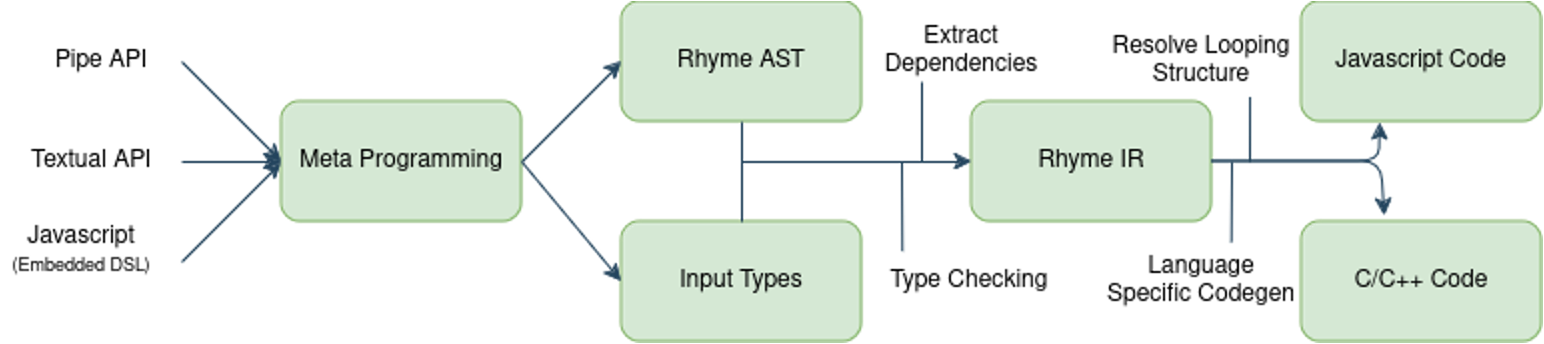
\includegraphics[scale=0.5]{figures/workflow.png}
      \caption{End-to-end workflow of \rhyme}
      \label{workflowfig}
  \end{figure}
\subsection{\rhyme Frontend}
\iffalse
\rhyme has multiple frontends like Pipe API, Textual API and Javascript API. \rhyme is a DSL embedded in Javascript, and as we mentioned before the \rhyme query can itself be a JSON object. Therefore we can use the JSON API to write query where the query is itself a JSON object. For example, if we want to group the sum of values of a dataset by its keys, we can just put \inline{data.*.key} as the key of the object query and put \inline{data.*.value} as the value as shown below. It is worth noting that since the \inline{sum(data.*.value)} is nested with \inline{data.*.key}, the logic variable in \inline{sum(data.*.value)} is bounded, the sum is actually a group-by sum. In addition to JSON API where the user can express the query in the same structure as the results, \rhyme also support Pipe API where the query is expressed as a sequence of transformations. The input wil pass through all the transformations to generate the final results. If we apply the logic variable \inline{.*} to a data source, the input will be iterated and a stream of its data will be passed for the following operation. The pipes are separated by \inline{|} symbol. The JSON API and Pipe API are equivalent and offers different ways to express the query for different application and scenarios. \par
\fi
\rhyme provides multiple frontends, including the Pipe API, Textual API, and JavaScript API. As a domain-specific language (DSL) embedded in JavaScript, \rhyme allows queries to be represented as JSON objects. This design enables users to construct queries directly in JSON format. For instance, to group the sum of values in a dataset by its keys, users can specify \inline{data.*.key} as the object query's key and \inline{data.*.value} as the value, as shown in the example below. Notably, because \inline{sum(data.*.value)} is nested within \inline{data.*.key}, the logic variable in \inline{sum(data.*.value)} is bound, making the operation a group-by sum.

In addition to the JSON API, where queries are expressed in the same hierarchical structure as their results, \rhyme also offers a Pipe API. The Pipe API allows queries to be defined as a sequence of transformations, where the input data passes through each transformation step to produce the final result. By applying the logic variable \inline{.*} to a data source, the input is iterated, and a stream of data is passed to subsequent operations. Transformations in the Pipe API are separated using the \inline{|} symbol.

The JSON API and Pipe API are equivalent in functionality but provide different methods for expressing queries, catering to various applications and scenarios.\par
\vspace*{1pt}
\noindent
\begin{minipage}{0.5\textwidth}\label{jsonapi}
\begin{lstlisting}
// JSON API: group the the sum of values by their keys
let query =  { data.*.key : sum(data.*.value) }
\end{lstlisting}
\end{minipage}%
\begin{minipage}{0.5\textwidth}
\begin{lstlisting}
//  Pipe API: group the sum of values by their keys
let key = rh`.data | .* | .key`
let query = rh`.data | .* | .value | group $\$${key}`
\end{lstlisting}
\end{minipage}
\vspace*{1pt}
\iffalse
The \rhyme query will be first parsed into an AST. The AST is a structured representation of the query and represented using JSON objects. \rhyme AST categorize operations into stateful operations (aggregation) and stateless operations (pure). The keys used for group-by will remain unchanged in the AST node. \rhyme will recursively translate the query into AST nodes and set the operator type and parameter correctly at each level.\par
In order to support generation of strongly typed languages like C/C++, \rhyme also allows user to provide optional type schemas of the input. As shown in Figure \ref{typeschema}, the user specify that the data is an object with u8 (8-bit unsigned integer) keys and string values. This type schema is crucial for our backend code generation as it provides type information for each sub-expressions of the query and allow us to generate more specialized code.
\fi
The \rhyme query is first parsed into an Abstract Syntax Tree (AST), a structured representation of the query expressed as JSON objects. The \rhyme AST categorizes operations into two types: stateful operations (e.g., aggregations) and stateless operations (e.g., pure functions). Keys used for group-by operations remain unchanged within the corresponding AST nodes. The \rhyme compiler recursively translates the query into AST nodes, assigning the appropriate operator types and parameters at each level.

To support code generation for strongly typed languages like C/C++, \rhyme allows users to optionally provide type schemas for the input data. As illustrated in Figure \ref{typeschema}, users can specify, for example, that the data consists of objects with 8-bit unsigned integer (u8) keys and string values. This type schema is essential for backend code generation, as it provides precise type information for each sub-expression of the query, enabling the generation of highly specialized and efficient code. We will talk about the type system more extensively in Section \ref{typesystem}.
\begin{figure}[H]
  \centering
      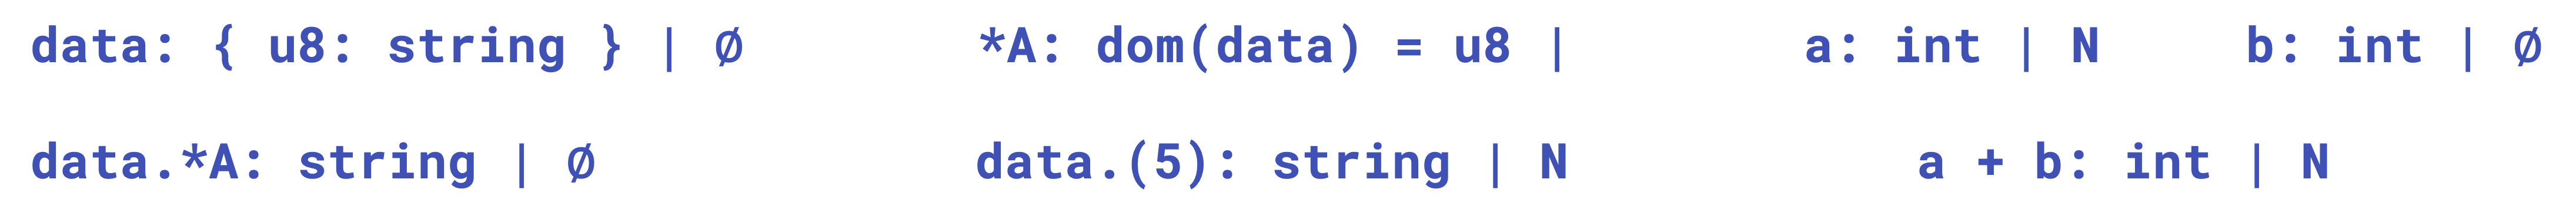
\includegraphics[scale=0.4]{figures/typeschema2.png}
      \caption{Example type schema of \rhyme}
      \label{typeschema}
  \end{figure}
\subsection{\rhyme Middle-end}
\iffalse
After the query is parsed into AST and the type schema is provided, we will perform type checking and inference and generate the intermediate representation. As shown in Figure \ref{typeschema}, we can infer the type of sub-expressions based on the given input type schema. If the input data has type \inline{{u8 : string}}, we can infer that the key of data \inline{*} (i.e. the logic variable) has type u8, we can also infer that \inline{data.*} has type string. We will perform both type inference and type checking to make sure that the type system conforms and we can correctly type all sub-expressions.\par
The \rhyme AST is a structured representation of the query, but we need a more fine-grained representation of the program that can capture both the data and control dependencies.
\rhyme has two types of IRs: \emph{generators} and \emph{assignments}. \emph{generators} are instructions used for iterating over a collection of data. Logic variables are responsible for iterating over data and directly map to generators. For example, \inline{data.*} corresponds to a generator that iterate over \inline{data}. \emph{assignments} are instructions used for computing the final and intermediate results. For example, \inline{sum(data.*)} corresponds to a sum operation that aggregate the value of \inline{data}.\rhyme also utilizes temporary variables to store materialized intermediate results.\par
It is worth noting that the IR does not enforce strict program structures. The program Structure is implied by the dependencies between statements. When an assignment uses a generator, it will cause a generator-assignment dependency (i.e. control dependency). When an assignment uses the result of an intermediate expression, it will cause a assignment-assignment dependency (i.e. data dependency). The \rhyme compiler will utilize these dependencies to produce an optimal program structure that respect the original query's semantic. Due to the dependencies-based IR design, \rhyme can perform multiple optimization like loop hoisting and code motion very easily.\par
After the IR generation, we will also assign types to each IR nodes. We will record the type of each generator and intermediate temporary variables. These type signature will be necessary when we generate code in the backend. We will also record for each generator the type of data sources they are iterating over. And we will generate specialized efficient code to co-iterate multiple data sources for one generator. For example, if one generator is co-iterating over multiple sparse vectors, we can generate specialized code to co-advancing the sparse vectors for efficiency as sparse vector does not offer constant-time look-up. We will cover this more in detail in Section \ref{sparse}.
\fi
After the query is parsed into an AST and the type schema is provided, \rhyme performs type checking and inference, followed by the generation of an intermediate representation (IR). As illustrated in Figure \ref{typeschema}, the type of sub-expressions can be inferred based on the input type schema. For example, if the input data is typed as \inline{\{u8 : string\}}, we can infer that the key of \inline{data} (i.e., the logic variable \inline{*}) has type \inline{u8}, while \inline{data.*} itself has type \inline{string}. Both type inference and type checking ensure that the type system is conformed and that all sub-expressions are correctly typed.

While the \rhyme AST provides a structured representation of the query, it is insufficient for capturing both data and control dependencies. For this purpose, \rhyme introduces two types of IRs: generators and assignments. Generators are instructions for iterating over data collections, with logic variables directly mapping to these generators. For example, \inline{data.*} corresponds to a generator that iterates over \inline{data}. Assignments, on the other hand, represent computations of intermediate and final results. For instance, \inline{sum(data.*)} corresponds to an aggregation operation that computes the sum of \inline{data} values. Temporary variables are also used to store materialized intermediate results.

The \rhyme IR does not enforce a rigid program structure; instead, the structure is implied by the dependencies between statements. A generator used by an assignment introduces a generator-assignment dependency (control dependency), while one assignment using the result of another creates an assignment-assignment dependency (data dependency). These dependencies guide the \rhyme compiler in generating an optimal program structure that preserves the original query semantics. This dependency-based IR design facilitates advanced optimizations such as loop hoisting and code motion.

Following IR generation, types are assigned to each IR node. The compiler records the types of generators and temporary variables, as well as the types of data sources associated with each generator. This type information is critical for backend code generation, enabling specialized and efficient co-iteration of multiple data sources. For example, if a generator co-iterates over multiple sparse vectors, \rhyme generates optimized code for advancing the sparse vectors efficiently, accounting for their lack of constant-time look-up. A more detailed explanation of these optimizations is provided in Section \ref{sparse}.
\subsection{\rhyme Backend}
\iffalse
\rhyme IR does not explicitly capture program dependencies, therefore we need to find an optimal program schedule for the query. We need to find an optimal loop schedule while respecting the correctness of program semantics. Since the IR nodes are only connected through dependencies, we need to figure out the order between loops, how loops should be nested and what instructions to put inside each loop. Putting code inside deeper loop nests could cause redundant computation and will even give us incorrect results if the code represents an aggregation. We also face exponential number of different choices of loop ordering and loop nests, each may cause different performance. We also want to maximize loop fusion such that assignments that depend on the same generator can be put inside one loop to reduce memory usage and loop control overhead. To achieve the goal mentioned above, we formalize the dependency constraints that the code generator needs to respect and derive a heuristic-based algorithm that can maximize loop fusion to ensure performance.\par
\rhyme has multiple backends such as JavaScript, C/C++. Therefore, our IR design is language-agonistic, we do not store any language-specific information in the IR. Instead, we only capture the core program relation (data and control dependencies) in the IR and different language backends can reuse the same dependency infrastructure. The IR nodes will also carry the type information to facilitate specialized cod generation. After the optimal program structure is scheduled, \rhyme will translate each IR nodes to the corresponding backend languages. \rhyme will also use the type information to generate the correct type signature and add explicit type cast when necessary.
\fi
The \rhyme IR does not explicitly encode program dependencies, making it necessary to derive an optimal program schedule for executing queries. This involves determining an optimal loop schedule while ensuring the correctness of the program semantics. Since the IR nodes are connected only through dependency relationships, the code generator must establish the order of loops, determine loop nesting, and decide which instructions to place inside each loop. Incorrectly placing code within deeper loop nests can lead to redundant computations or, in cases involving aggregations, even incorrect results.

The challenge is further compounded by the exponential number of possible loop orderings and nesting configurations, each with varying performance characteristics. To improve performance, it is also essential to maximize loop fusion, enabling assignments dependent on the same generator to be placed within a single loop. This minimizes memory usage and loop control overhead.

To address these challenges, we formalize the dependency constraints that the code generator must respect and design a heuristic-based algorithm that prioritizes loop fusion. This approach ensures both performance optimization and semantic correctness.

\rhyme supports multiple backends, including JavaScript and C/C++. To maintain flexibility, the IR is designed to be language-agnostic and excludes any language-specific details. Instead, it captures only the core program relationships—data and control dependencies. This allows different backends to reuse the same dependency-based IR infrastructure. Each IR node also carries type information to facilitate specialized code generation.

Once an optimal program structure is determined, \rhyme translates the IR nodes into code for the target backend language. During this translation, the type information is used to generate accurate type signatures and insert explicit type casts where necessary. This ensures the generated code is both correct and efficient for the specific backend.\par
\section{Type System}\label{typesystem}
\iffalse
In the section, we will dive deep into the type system and type checking/inference algorithms for \rhyme. Formally, the type id defined as sets of possible values. And we have a \emph{Any} type $\top$ which represents the universal set of all possible values, and a \emph{Never} type $\bot$ which represents the empty set. These serve as the top and bottom of our type lattice. \rhyme has multiple primitive types:
\begin{itemize}
  \item \emph{Number type}: \rhyme has unsigned integer $U$, signed integer $I$ and floating point numbers $F$ as primitive number type, $N = U \cup I \cup F$.\begin{itemize}
    \item Unsigned integer: $U = \{ u8, u16, u32, u64 \}$
    \item Signed integer: $I = \{ i8, i16, i32, i64 \}$
    \item Floating point: $F = \{ f32, f64 \}$
  \end{itemize}
  \item \emph{String type}: String is a native type in \rhyme system and represents the set of all strings.
  \item \emph{Tensor type}: \rhyme supports both sparse and dense tensor algebra, therefore we also support tensor types. $T = <\text{mode}, \text{dims}, \text{elemTy}>$, tensor types are a tuple: \begin{itemize}
    \item mode: mode represents whether the tensor is sparse or dense.
    \item dims: dims record the dimensions of tensor, \rhyme allows arbitrary dimension tensors.
    \item elemTy: elemTy records the elemTy of a Tensor, it can be any number types.
  \end{itemize}
  \item \emph{Object type}: \rhyme supports object types, object types itself is also an object where the key is the key type and value is the value type. For example, \inline{{u8: string}} is a valid object type.
  \item \emph{Key type}: key types can represent the set of keys for certain object. Since different objects may have different domains, even though their key type is the same (for example, both i32), their key domains may not be the same. Therefore, we also a key type, $K_n(T)$ representing the exact key set of an object.
  \item \emph{Nothing type and Error type}: An expression can produce no values or throw an error (divide by zero). We want to propagate these information as much as we can. Therefore, \rhyme also includes both the \emph{Nothing} ($\mathcal{N}$) and \emph{Error} ($\mathcal{E}$) type.
\end{itemize}
\fi
In this section, we delve into the type system and the type checking/inference algorithms for \rhyme. Formally, a type is defined as a set of possible values. We define an \emph{Any} type $\top$, representing the universal set of all possible values, and a \emph{Never} type $\bot$, representing the empty set. These serve as the top and bottom elements of the type lattice, respectively.
\subsection{Primitive Types}
\rhyme supports multiple primitive types:

\begin{itemize} \item \textbf{Number type}: \rhyme includes unsigned integers ($U$), signed integers ($I$), and floating-point numbers ($F$) as primitive numeric types, collectively represented as $N = U \cup I \cup F$. \begin{itemize} \item Unsigned integers: $U = { u8, u16, u32, u64 }$ \item Signed integers: $I = { i8, i16, i32, i64 }$ \item Floating-point numbers: $F = { f32, f64 }$ \end{itemize}

\item \textbf{String type}: Strings are a native type in the \rhyme system and represent the set of all possible strings.

\item \textbf{Tensor type}: To support both sparse and dense tensor algebra, \rhyme introduces tensor types, denoted as $T = \langle \emph{mode}, \emph{dims}, \emph{elemTy} \rangle$. A tensor type is a tuple consisting of: \begin{itemize} \item \emph{mode}: Indicates whether the tensor is sparse or dense. \item \emph{dims}: Represents the dimensions of the tensor; \rhyme supports tensors with arbitrary dimensions. \item \emph{elemTy}: Specifies the element type of the tensor, which can be any number type. \end{itemize}

\item \textbf{Object type}: \rhyme supports object types, where an object type is itself an object defined by key-value pairs. The key specifies the key type, and the value specifies the value type. For example, \inline{\{u8: string\}} is a valid object type.

\item \textbf{Key type}: Key types represent the set of keys for specific objects. Since objects may have different key domains, even if their key types are identical (e.g., both are $i32$), the specific key domains may differ. To handle this, \rhyme includes a key type $K_n(T)$, representing the exact key set of an object.

\item \textbf{Nothing type and Error type}: An expression can produce no values (e.g., in cases of empty results) or throw an error (e.g., division by zero). To propagate this information, \rhyme includes the \emph{Nothing} type ($\mathcal{N}$) and the \emph{Error} type ($\mathcal{E}$). \end{itemize}
\subsection{Union Type and Intersection Type}
\iffalse
\rhyme also supports union type and intersection type.
\begin{itemize}
  \item \textbf{Union type}: Since an expression can produce either a valid result or an error and we want to propagate the error message. We support union type to carry the additional \emph{Error type} in the result type. For example, a 32-bit floating point division's result will have type $f32 \cup \mathcal{E}$ which means the result is either a 32 bit floating point number or an error.
  \item \textbf{Intersection Type}: Since a generator can iterate over multiple data sources, and different data sources may have different domains, the type of the generator is the intersection of the types of the input domains. For example, if we have both $A.*$ and $B.*$ in one query, and the key type of $A$ is $K_a$, the key type of $B$ is $K_b$. The type of the generator $*$ is $K_a \cap K_b$.
\end{itemize}
\fi
\rhyme also supports union types and intersection types:

\begin{itemize} \item \textbf{Union type}: Since an expression can produce either a valid result or an error, and we want to propagate the error message, \rhyme supports union types to include the \emph{Error type} in the result type. For example, the result of a 32-bit floating-point division will have the type $f32 \cup \mathcal{E}$, indicating that the result is either a 32-bit floating-point number or an error.

\item \textbf{Intersection type}: When a generator iterates over multiple data sources, and those data sources have different domains, the generator's type is the intersection of the input domain types. For instance, if a query involves both $A.\ast$ and $B.\ast$, where the key type of $A$ is $K_a$ and the key type of $B$ is $K_b$, the type of the generator $\ast$ is $K_a \cap K_b$. \end{itemize}
\subsection{Subtyping}
\iffalse
We also support subtyping in our type system since we support multiple bits numbers, union type, intersection type. Let the subtype relation be The subtype rules for \rhyme are pretty straight forward and are listed below.\par
\noindent
\begin{minipage}{0.5\textwidth}
\begin{figure}[H]
  \centering
$u8 \leq: u16 \leq: u32 \leq: u64$\par
\vspace*{2mm}
$i8 \leq: i16 \leq: i32 \leq: i64$\par
\vspace*{2mm}
$f32 \leq: f64$, $u8 \leq: i16$, $u16 \leq: i32$, $u32 \leq: i64$\par
\vspace*{2mm}
$i16 \leq: f32$, $u16 \leq: f32$\par
\vspace*{2mm}
$i32 \leq: f64$, $u32 \leq: f64$
\caption*{Number type subtyping rules}
\end{figure}
\end{minipage}
\begin{minipage}{0.5\textwidth}
  \centering
\begin{figure}[H]
$\inference {} {|- T \leq: \top}$ \hspace*{10mm} $\inference {} {|- \bot \leq: T}$\par
\vspace*{4mm}
$\inference {\Gamma |- x: T \quad |- T \leq: S}{\Gamma |- x: S}$ \hspace*{4mm}
$\inference {}{|- T \leq: T}$\par
\vspace*{4mm}
$\inference {|- T \leq: S \quad |- S \leq: T}{|- S =: T}$
$\inference {|- S =: T}{|- T \leq: S \quad |- S \leq: T}$
\caption*{Basic subtyping rules}
\end{figure}
\end{minipage}
\begin{minipage}{0.5\textwidth}
\begin{figure}[H]
  \centering
\vspace*{5mm}
$\inference {}{|- T \leq: (T \cup S)}$\hspace*{2mm}
$\inference {}{|- (S \cup T) =: (T \cup S)}$\par
\vspace*{4mm}
$\inference {}{|- (T \cup T) =: T}$\hspace*{2mm}
$\inference {|- T \leq: S}{|- (T \cup S) =: S}$
\caption*{Union type subtyping rules}
\end{figure}
\end{minipage}
\begin{minipage}{0.5\textwidth}
\begin{figure}[H]
  \centering
\vspace*{5mm}
$\inference {\Gamma |- t : T \quad \Gamma |- t : S}{\Gamma |- t : (T \cap S)}$\hspace*{2mm}
$\inference {}{|- (T \cap S) \leq: T}$\par
\vspace*{4mm}
$\inference {}{|- (S \cap T) =: (T \cap S)}$\hspace*{2mm}
$\inference {}{|- (T \cap T) =: T}$\par
\vspace*{4mm}
$\inference {|- T \leq: S}{|- (T \cap S) =: T}$
\caption*{Intersection type subtyping rules}
\end{figure}
\end{minipage}
\subsection{Type checking and inference}
After the input type schema is passed, \rhyme will perform type inference and type checking to make sure the type schema is conformed and we can assign a valid type for each sub expression. We will infer the type of all sub expressions from the given type schema. We will iteratively perform type infer using existing knowledge while perform type checking and lifting to ensure correctness. The type inference and checking algorithms work on the following statements:
\begin{itemize}
  \item \textbf{Stateful operations}: If we know the type of $a$ is $T$, we know that the aggregation of $a$ has the same type. It is worth noting that even if $T$ is a union type that carry \emph{Nothing type} $\mathcal{N}$, the aggregation of $a$ may not carry the \emph{Nothing type} as aggregations (like sum) have an initial value and may skip over empty values.
  \item \textbf{Pure operations}: On pure operations like plus or multiplication, \rhyme will first infer the type of its operands, and use the super type of its operands' type as its type. \rhyme will also keep track of the error conditions like \emph{Nothing type} and \emph{Error type} in the operands and propagate them upwards. \rhyme backend will also add explicit type cast if an operand is lifted to its super type, for example, if we add \inline{u8} with \inline{u32}, we need to cast the first operand to \inline{u32}.
  \item \textbf{Generators}: We will also infer the type of generators from the type schema of the data sources it iterates over. As we mentioned above, the generator's type is the intersection of the key type of its data sources. For example, if we know \inline{input} is a 1-D dense tensor with \inline{i32} elements, and we apply the generator \inline{*} to it. We know that the type of \inline{*} is \inline{u32} and the type of \inline{input.*} is \inline{i32}. We also know that \inline{*} is in a continuous range, so we can just increment \inline{*} by one for iteration. This may not be the case for sparse tensors.
\end{itemize}
\fi
We also support subtyping in our type system, which is essential for handling multiple bit-width numbers, type casting, union types, and intersection types. Let the subtype relation be $\leq:$, the subtype rules for \rhyme are outlined below.\par
\noindent
\begin{minipage}{0.5\textwidth}
\begin{figure}[H]
  \centering
$u8 \leq: u16 \leq: u32 \leq: u64$\par
\vspace*{2mm}
$i8 \leq: i16 \leq: i32 \leq: i64$\par
\vspace*{2mm}
$f32 \leq: f64$, $u8 \leq: i16$, $u16 \leq: i32$, $u32 \leq: i64$\par
\vspace*{2mm}
$i16 \leq: f32$, $u16 \leq: f32$\par
\vspace*{2mm}
$i32 \leq: f64$, $u32 \leq: f64$
\caption*{Number type subtyping rules}
\end{figure}
\end{minipage}
\begin{minipage}{0.5\textwidth}
  \centering
\begin{figure}[H]
$\inference {} {|- T \leq: \top}$ \hspace*{10mm} $\inference {} {|- \bot \leq: T}$\par
\vspace*{4mm}
$\inference {\Gamma |- x: T \quad |- T \leq: S}{\Gamma |- x: S}$ \hspace*{4mm}
$\inference {}{|- T \leq: T}$\par
\vspace*{4mm}
$\inference {|- T \leq: S \quad |- S \leq: T}{|- S =: T}$
$\inference {|- S =: T}{|- T \leq: S \quad |- S \leq: T}$
\caption*{Basic subtyping rules}
\end{figure}
\end{minipage}
\begin{minipage}{0.5\textwidth}
\begin{figure}[H]
  \centering
\vspace*{5mm}
$\inference {}{|- T \leq: (T \cup S)}$\hspace*{2mm}
$\inference {}{|- (S \cup T) =: (T \cup S)}$\par
\vspace*{4mm}
$\inference {}{|- (T \cup T) =: T}$\hspace*{2mm}
$\inference {|- T \leq: S}{|- (T \cup S) =: S}$
\caption*{Union type subtyping rules}
\end{figure}
\end{minipage}
\begin{minipage}{0.5\textwidth}
\begin{figure}[H]
  \centering
\vspace*{5mm}
$\inference {\Gamma |- t : T \quad \Gamma |- t : S}{\Gamma |- t : (T \cap S)}$\hspace*{2mm}
$\inference {}{|- (T \cap S) \leq: T}$\par
\vspace*{4mm}
$\inference {}{|- (S \cap T) =: (T \cap S)}$\hspace*{2mm}
$\inference {}{|- (T \cap T) =: T}$\par
\vspace*{4mm}
$\inference {|- T \leq: S}{|- (T \cap S) =: T}$
\caption*{Intersection type subtyping rules}
\end{figure}
\end{minipage}

\subsection{Type Checking and Inference} Once the input type schema is provided, \rhyme performs type inference and type checking to ensure that the type schema conforms and that valid types can be assigned to all sub-expressions. The algorithm iteratively infers types based on existing information while performing type checking and lifting to maintain correctness. The type inference and checking algorithms operate on the following constructs:

\begin{itemize} \item \textbf{Stateful operations}: If the type of $a$ is $T$, then the aggregation of $a$ has the same type $T$. Note that even if $T$ is a union type that includes the \emph{Nothing type} $\mathcal{N}$, the aggregation of $a$ may not propagate the \emph{Nothing type} because aggregations (e.g., \texttt{sum}) use an initial value and may skip empty entries.

\item \textbf{Pure operations}: For pure operations like addition or multiplication, \rhyme infers the types of the operands and assigns the supertype of the operands' types as the result type. Additionally, \rhyme tracks error conditions such as the \emph{Nothing type} and \emph{Error type} in the operands and propagates them upward. If an operand is lifted to its supertype, the backend adds explicit type casts where necessary. For example, adding \inline{u8} to \inline{u32} requires casting the first operand to \inline{u32}.

\item \textbf{Generators}: Generator types are inferred based on the type schema of the data sources they iterate over. As mentioned earlier, the generator's type is the intersection of the key types of its data sources. For instance, if \inline{input} is a 1-D dense tensor with \inline{i32} elements and the generator \inline{*} is applied, the type of \inline{*} is \inline{u32}, and the type of \inline{input.*} is \inline{i32}. Since \inline{*} iterates over a continuous range, it can be incremented by one for each iteration. However, this is not guaranteed for sparse tensors. \end{itemize}\par
\iffalse
\rhyme 's type system lays the foundations for specialized code generation for strongly typed languages like C/C++ as well as sparse tensor algebra. Dense tensor and sparse tensor has different characteristics and require different methods for both data loading as well as efficient co-iteration. We will cover how this type system facilitates efficient code generation for Sparse Tensor Algebra in the next section.
\fi
\rhyme's type system forms the foundation for specialized code generation for strongly typed languages like C/C++ as well as for sparse tensor algebra. Dense tensors and sparse tensors have distinct characteristics, requiring different strategies for both data loading and efficient co-iteration. In the next section, we will discuss how this type system supports the efficient code generation of sparse tensor algebra.
\section{Sparse Tensor Algebra}\label{sparse}
\iffalse
In this section, we will discuss how \rhyme supports specialized code generation for sparse tensor algebra and how it manage to efficiently co-iterate over sparse tensors inside a multi-paradigm framework.\par
As we mentioned in Section \ref{introduction}, sparse tensor is widely used in both scientific computation and machine learning applications. Existing approach either uses hand written kernels to execute sparse tensor algebra or develops a sparse tensor compiler to automatically generate code given the tensor computation notations. However, integrating efficient sparse tensor algebra with relational algebra into a declarative language framework still remains a challenging problem. \rhyme manages to support efficient code generation for sparse tensor algebra inside a unified multi-paradigm framework.\par
Sparse tensor code generation reuses the same IR and dependency analysis pass as other domains, as the data and control dependencies are the same as dense tensor computation. After the user provides type schema indicating that the input is a sparse tensor, we will perform type inference and checking to assign valid types to all sub-expressions and intermediate temporary variables. We will also generate specialized functions to read/load the sparse tensor into memory as the sparse tensors are different format than dense formats. We support compressed notations of sparse vectors, where the non-zero values and their corresponding indexes are stored. Due to the sparsity nature of the data, sparse data does not offer constant-time look-up as the indexes stored are not continuous, a binary search will need to be taken to check existence of an index. Although sparse tensors does not offer constant-time random-access, it reduces the memory storage by only storing the non-fill (non-zero) elements. This compressed format also offers the opportunity for a more efficient way of computing tensors as the computation on zero elements can be skipped and we only need to compute for non-zero elements. For example, if we compute a dot product of two sparse vectors, we only need to multiply the indexes that all non-zero in both vectors.\par
\fi
In this section, we discuss how \rhyme supports specialized code generation for sparse tensor algebra and how it efficiently co-iterates over sparse tensors within a multi-paradigm framework.\par
As mentioned in Section \ref{introduction}, sparse tensors are widely used in both scientific computation and machine learning applications. Existing approaches either rely on hand-written kernels for executing sparse tensor algebra or develop sparse tensor compilers to automatically generate code from tensor computation notations. However, integrating efficient sparse tensor algebra with relational algebra into a declarative language framework remains a significant challenge. \rhyme addresses this challenge by enabling efficient code generation for sparse tensor algebra within a unified multi-paradigm framework.\par
Sparse tensor code generation in \rhyme reuses the same IR and dependency analysis passes as other domains, as the data and control dependencies for sparse tensors are identical to those for dense tensor computations. When the user provides a type schema indicating that the input is a sparse tensor, \rhyme performs type inference and checking to assign valid types to all sub-expressions and intermediate temporary variables. Additionally, \rhyme generates specialized functions to read and load sparse tensors into memory, as their storage format differs from dense tensor formats.\par
\rhyme supports compressed representations of sparse vectors, where only the non-zero values and their corresponding indices are stored. Due to the sparse nature of the data, sparse tensors do not offer constant-time look-up because the stored indices are not continuous. A binary search is required to check the existence of an index. While sparse tensors lack constant-time random access, they significantly reduce memory usage by storing only the non-fill (non-zero) elements. This compressed format also provides an opportunity for more efficient computations, as operations on zero elements can be skipped, and computations are performed only on non-zero elements. For example, when computing the dot product of two sparse vectors, it is sufficient to multiply the elements corresponding to indices that are non-zero in both vectors.
\subsection*{Efficient co-iteration of sparse vectors}
\iffalse
Different sparsity patterns require different ways of iterating tensors, and it is non-trivial to pick the best strategy, it also adds another layer of complexity to \rhyme's loop scheduling algorithm. Originally, if a generator iterates over multiple inputs, \rhyme will generate only one loop to iterate over one of the inputs and check whether the key exists for the remaining inputs. However, in the face of sparse tensor algebra, this naive loop co-iteration algorithm may yield suboptimal performance.\par
For example, if we are performing a dot product of a sparse vector $A$ and dense vector $B$. And assume that $A$ has $m$ non-zero elements and is stored in a compressed format, and $B$ has $n$ elements. If we choose to loop over $A$ first and check existence in $B$, the computation only takes $\Theta(m)$ complexity as existence checks in dense vector takes constant time. However, if we choose to loop over $B$ first and check existence in $A$, the computation will take $\Theta(n\log{}m)$, as existence checks in sparse vector takes logarithmic time at best. This simple example shows that careless selection of co-iteration strategies in dense/sparse tensor algebra could greatly downgrade the performance.\par
The complexity continues to rise if we consider co-iteration of multiple sparse tensors. When we iterate over multiple sparse tensors, picking one sparse tensor to loop over and check existence in others will yield suboptimal performance regardless of the tensor we choose to loop over. For example, if we are performing a dot product of a sparse vector $A$ and sparse vector $B$. And assume that $A$ has $m$ non-zero elements and is stored in a compressed format, and $B$ has $n$ non-zero elements and is stored in a compressed format. And assume that the non-zero indices stored in both tensors are sorted. If we pick to loop over $A$ first and check existence in $B$, the computation will take $\Theta(m\log{}n)$ assuming we use binary search. If we pick to loop over $B$ first, the computation will take $\Theta(n\log{}m)$. However, an efficient co-iteration strategy (the two-way merge algorithm \cite{knuth}) that advancing indices in $A$ and $B$ together only need $O(m + n)$ time. This is much more efficient especially if $m$ and $n$ are at the same scale. It should be noted that we are talking about the strategy for multiplication here where all operands need to be non-zero for the result to be non-zero. Addition on the other hand will require a similar but different co-iteration strategy.\par
The N-way merge algorithm works by assigning pointers to each sparse vectors, each starting at the first non-zero indices. Then we will compare the indices in all the sparse vectors and only execute the computation when all the indices are the same, which means this index has non-zero value in all sparse vectors. If the indices are not the same, we can advance the pointer of the sparse vector that has the smallest index and that index can be skipped. We can also find the largest index among the pointers and advance all other pointers until their pointers point to indices larger or equal to the current largest index. The rationale is that all the indices smaller that the current max index must not exist in all sparse vectors, therefore can be skipped. We will apply this strategy iteratively until one of the sparse vectors runs out of value.\par
\rhyme compiler will pick an efficient strategy for different co-iteration generators depending on the dense/sparse patterns of the data sources. Combing this with the loop scheduling and fusion optimization that \rhyme's original backend offers, we can generate efficient code for sparse tensor algebra inside a multi-paradigm language framework.
\fi
Different sparsity patterns require different methods for iterating over tensors, making it non-trivial to select the best strategy. This adds an additional layer of complexity to \rhyme's loop scheduling algorithm. Originally, when a generator iterates over multiple inputs, \rhyme generates a single loop to iterate over one input and checks for the existence of corresponding keys in the remaining inputs. However, in the context of sparse tensor algebra, this naive co-iteration approach may result in suboptimal performance.\par
For example, consider the dot product of a sparse vector $A$ and a dense vector $B$. Assume that $A$ has $m$ non-zero elements stored in a compressed format, and $B$ has $n$ elements. If we loop over $A$ and check for the existence of indices in $B$, the computation takes $\Theta(m)$ time because existence checks in a dense vector occur in constant time. Conversely, if we loop over $B$ and check for the existence of indices in $A$, the computation takes $\Theta(n\log{}m)$ time because existence checks in a sparse vector require logarithmic time due to the use of binary search. This example highlights how an inappropriate co-iteration strategy can significantly degrade performance in dense/sparse tensor algebra.\par
The complexity further escalates when co-iterating over multiple sparse tensors. Simply choosing one sparse tensor to iterate over and checking for existence in others will generally yield suboptimal performance. For instance, consider the dot product of two sparse vectors $A$ and $B$. Suppose $A$ has $m$ non-zero elements and $B$ has $n$ non-zero elements, both stored in compressed formats with sorted indices. If we loop over $A$ and check existence in $B$, the computation requires $\Theta(m\log{}n)$ time using binary search. Similarly, looping over $B$ and checking in $A$ requires $\Theta(n\log{}m)$ time. However, an efficient co-iteration strategy, such as the two-way merge algorithm \cite{knuth}, advances indices in $A$ and $B$ together and achieves a time complexity of $O(m + n)$. This strategy is especially advantageous when $m$ and $n$ are of comparable scales. Note that this strategy applies to multiplication operations, where all operands must be non-zero for the result to be non-zero. For addition operations, a similar but distinct co-iteration strategy is required.\par
The N-way merge algorithm addresses co-iteration by assigning pointers to each sparse vector, starting at their respective first non-zero indices. The algorithm compares indices across all sparse vectors, executing the computation only when the all indices are the same (indicating non-zero values in all vectors at this index). If the indices do not match, the pointer of the vector with the smallest index is advanced, skipping that index. Alternatively, the algorithm can identify the largest index among the current pointers and advance all other pointers to indices greater than or equal to the largest index. This optimization skips indices that cannot exist in all sparse vectors. The process repeats iteratively until one of the sparse vectors is exhausted.\par
The \rhyme compiler selects an efficient co-iteration strategy for different generators based on the sparsity patterns of the data sources. Combined with \rhyme's backend loop scheduling and fusion optimizations, this approach enables the specialized generation of high-performance code for sparse tensor algebra within a multi-paradigm language framework.
\subsection*{Implementation}
\iffalse
\rhyme currently implements a C++ backend for sparse tensor algebra. As \rhyme 's type system supports multiple-width integers and floating point numbers, to maximize code reuse, we heavily utilize template in C++ to achieve polymorphism. We also utilize template meta-programming to simplify the functions used for sparse/dense tensor loading. We implement the compressed matrix and vector data structures in a C++ header. The data structure are also polymorphic and supports both the index type and value type to be template parameters.\par
We also implemented custom \emph{multi\_iterator} class used to specifically perform efficient co-iteration of multiple sparse vectors. It utilizes the N-way merge algorithm we mentioned before. Upon initialization, it takes a list of sparse vectors as arguments, and initialize the N-way merge algorithm. We overload the dereference $\ast$ operator and the increment ++ operator. So that the ++ operator will co advance the pointers in the sparse vectors until indices in all sparse vectors are the same.  The $\ast$ operator will output a pair containing the index and the list of values at this index for sparse vectors.\par
After the C++ code is generated, the host compiler like gcc or clang can be used to compile and optimize the program for execution.
\fi
\rhyme currently implements a C++ backend for sparse tensor algebra. Since \rhyme's type system supports multiple-width integers and floating-point numbers, we leverage templates in C++ to achieve polymorphism and maximize code reuse. Additionally, we utilize template metaprogramming to simplify the functions used for loading sparse and dense tensors. Compressed matrix and vector data structures are implemented in a C++ header file. These data structures are polymorphic, with both the index type and value type defined as template parameters.\par
We have also implemented a custom \emph{multi\_iterator} class specifically designed for efficient co-iteration of multiple sparse vectors. This class employs the N-way merge algorithm discussed earlier. Upon initialization, it takes a list of sparse vectors as arguments and sets up the N-way merge algorithm. The class overloads the dereference ($\ast$) operator and the increment (++) operator. The ++ operator advances the pointers in the sparse vectors until the indices in all vectors are the same, while the $\ast$ operator returns a pair consisting of the current index and a list of values at that index for the sparse vectors.\par
Once the C++ code is generated, it can be compiled and optimized for execution using host compilers such as GCC or Clang.
\section{Evaluation}\label{evaluation}
\iffalse
In this section, we will compare our generated code for sparse tensor algebra with the state of the art sparse tensor compiler TACO. We will compare the generated code and execute them to compare the performance.\par
We use a simple tensor computation to compare the generated code - dot product of 4 sparse vectors. The mathematical definition of the computation is given below:
$$A = \sum_{i} B_i \cdot C_i \cdot D_i \cdot E_i$$
The query of this tensor computation for \rhyme and TACO are listed below:\par
\fi
In this section, we will compare the code generated by \rhyme for sparse tensor algebra with the state-of-the-art sparse tensor compiler, TACO. We will analyze the generated code and execute it to evaluate performance.\par
We use a simple tensor computation to compare the generated code: the dot product of four sparse vectors. The mathematical definition of this computation is given below:
$$A = \sum_{i} B_i \cdot C_i \cdot D_i \cdot E_i$$
The queries for this tensor computation in \rhyme and TACO are listed below:\par
\vspace*{2mm}
\begin{minipage}{0.5\textwidth}
\begin{lstlisting}[basicstyle=\ttfamily\footnotesize]
// Rhyme query
rh`sum(B.*i * C.*i * D.*i * E.*i)`
\end{lstlisting}
\end{minipage}%
\begin{minipage}{0.5\textwidth}
\begin{lstlisting}[basicstyle=\ttfamily\footnotesize]
// TACO query
A = B(i) * C(i) * D(i) * E(i)
\end{lstlisting}
\end{minipage}

\vspace*{2mm}
\noindent
We will also provide additional type schema for the \rhyme query, indicating that the 4 vectors are sparse. The query will go through the type inference/checking, IR-generation, loop scheduling and code generation phase as we mentioned in Section \ref{workflow}. The final generated code for \rhyme and TACO are shown below (we only show the computation code and excluded the data loading and driver code).\par
\vspace*{2mm}
\noindent
\begin{lstlisting}[basicstyle=\ttfamily\footnotesize]
// Rhyme generated code
int tmp0 = 0;
for (auto xi_mit = CSVector<int, int>::multi_iterator({&B,&C,&D,&E});!xi_mit.finish(); ++xi_mit) {
  tmp0 += (int)(((*xi_mit).second[0] * (*xi_mit).second[1] * (*xi_mit).second[2] * (*xi_mit).second[3]));
}
\end{lstlisting}

\vspace*{2mm}

\begin{lstlisting}[basicstyle=\ttfamily\footnotesize]
// TACO generated code
while (((i204B < pB1_end && i204C < pC1_end) && i204D < pD1_end) && i204E < pE1_end) {
  int32_t i204B0 = B1_crd[i204B];
  int32_t i204C0 = C1_crd[i204C];
  int32_t i204D0 = D1_crd[i204D];
  int32_t i204E0 = E1_crd[i204E];
  int32_t i204 = TACO_MIN(i204B0,TACO_MIN(i204C0,TACO_MIN(i204D0,i204E0)));
  if (((i204B0 == i204 && i204C0 == i204) && i204D0 == i204) && i204E0 == i204) {
    A0_val += ((B_vals[i204B] * C_vals[i204C]) * D_vals[i204D]) * E_vals[i204E];
  }
  i204B += (int32_t)(i204B0 == i204);
  i204C += (int32_t)(i204C0 == i204);
  i204D += (int32_t)(i204D0 == i204);
  i204E += (int32_t)(i204E0 == i204);
}
\end{lstlisting}
\vspace*{2mm}
\iffalse
As we can observe, \rhyme 's generated code is more simple and can be directly mapped to the original query. \rhyme heavily utilize C++'s template feature and operator overloading to make the generated code more declarative and easy to understand. We also preserve the iteration logic in the original query by using the custom multi\_iterator. All the complex logic for co-advancing pointers in hidden in the header files.\par
\fi
As we can observe, \rhyme's generated code is simpler and can be directly mapped to the original query. \rhyme heavily utilizes C++'s template features and operator overloading to make the generated code more aligned with the original query logic and easier to understand. The iteration logic from the original query is preserved by using the custom \emph{multi\_iterator}. All the complex logic for co-advancing pointers is encapsulated within the header files.\par
\begin{figure}[H]
  \centering
      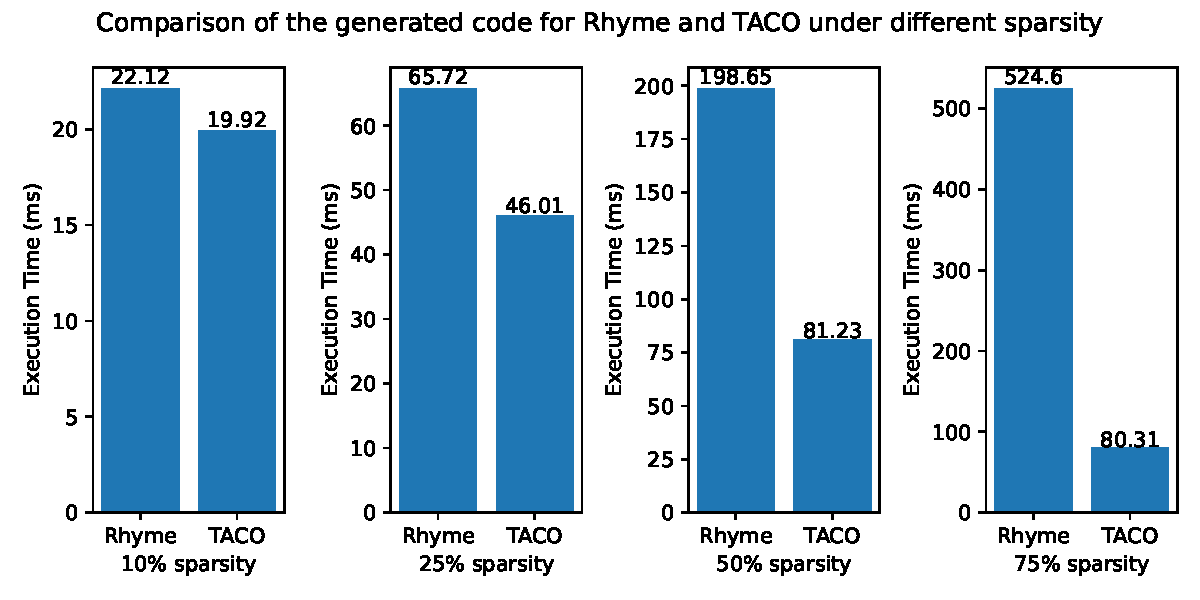
\includegraphics[scale=0.7]{figures/evaluation.pdf}
      \caption{\rhyme vs TACO}
      \label{evaluationpic}
  \end{figure}
\iffalse
We also compared the execution time of \rhyme and TACO, we run the generated code on 4 randomly generated sparse vectors with 10 percent sparsity. The result is shown in Figure \ref{evaluationpic}. As we can observe, \rhyme 's generated code can achieve roughly $86\%$ performance of TACO in the example query. The performance gap could be caused by the fact that TACO generates native C code for the computation kernel while our header file is purely written in C++ and heavily utilize STL containers. Our backend also adds several abstractions over both the sparse tensor data structure and the co-iteration method which could add additional overhead. But it should be noted that \rhyme is still an ongoing project and we could develop a pure C backend and generate more specialized C code with not much development effort. Also, compared with TACO, \rhyme manage to integrate relational algebra with sparse tensor algebra in a unified framework and perform several loop optimization likes loop hoisting and fusion.
\fi
We also compared the execution time of \rhyme and TACO by running the generated code on four randomly generated sparse vectors with the same sparsity. The experiment was conducted with varying degrees of sparsity (10$\%$, 25$\%$, 50$\%$, and 75$\%$). Sparsity is defined as the ratio of non-zero values to all values. The results are shown in Figure \ref{evaluationpic}. As observed, \rhyme's generated code achieves approximately $90\%$ of TACO's performance at 10$\%$ sparsity for the example query. However, as sparsity increases, \rhyme's performance declines relative to TACO. At 75$\%$ sparsity, \rhyme achieves only $15\%$ of TACO's performance.\par
The performance gap may stem from several factors. First, TACO generates native C code for its computation kernel, whereas \rhyme's backend relies on C++ and heavily utilizes STL containers. Additionally, \rhyme introduces several abstractions over both the sparse tensor data structure and the co-iteration method implemented in the header file, which likely contribute to additional overhead. Moreover, \rhyme employs a different co-advancing algorithm than TACO. While TACO increments only the smallest pointer at each iteration, \rhyme identifies the largest pointer and advances all other pointers until their indices become greater than or equal to the current largest pointer. This may explain why the performance gap decreases as the vectors become sparser.\par
It is important to note that \rhyme is still an ongoing project, and performance is not the primary focus at this stage. With minimal development effort, we could implement a pure C backend to generate more specialized C code, reducing the overhead of C++ abstractions and STL containers. Additionally, we could adopt TACO's co-iteration logic as an alternative implementation in our header. Our primary contribution lies not in the already well-established area of sparse tensor computation kernels, but in efficiently integrating sparse tensor algebra within a declarative multi-paradigm language framework. Existing optimized co-iteration logic can easily be incorporated into our implementation. Furthermore, compared to TACO, \rhyme integrates relational algebra and sparse tensor algebra into a unified framework while supporting advanced loop optimizations, such as loop hoisting and fusion.
\section{Conclusion}\label{conclusion}
\iffalse
In this paper, we present \rhyme - a declarative multi-paradigm query language that support both relational algebra and dense/sparse tensor algebra in a unified framework. We give a detailed explanation of how \rhyme supports specialized code generation for sparse tensor algebra and its type system design. \rhyme is still under development and we believe with more development effort, \rhyme can support multi-paradigm workload efficiently.
\fi
In this paper, we present \rhyme—a declarative multi-paradigm query language that supports both relational algebra and dense/sparse tensor algebra within a unified framework. We provide a detailed explanation of how \rhyme enables specialized code generation for sparse tensor algebra and the design of its type system. While \rhyme is still under active development, we believe that, with further effort, it can efficiently support multi-paradigm workloads.
%\newpage
\bibliographystyle{acm}
\bibliography{paper}
\end{document}
\endinput
